\documentclass{standalone}
\usepackage{tikz}
\usetikzlibrary{arrows.meta}

\begin{document}

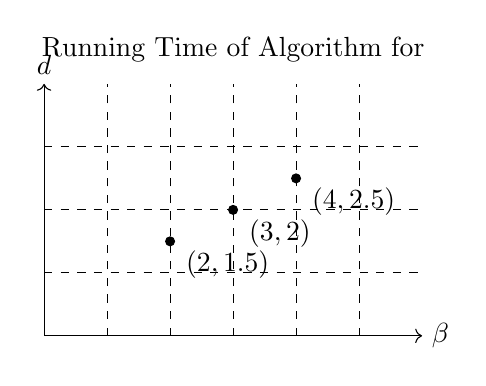
\begin{tikzpicture}[scale=0.8]
    % Define axes
    \draw[->] (0,0) -- (6,0) node[right] {$\beta$};
    \draw[->] (0,0) -- (0,4) node[above] {$d$};

    % Draw grid lines
    \foreach \x in {1,...,5} {
        \draw[dashed] (\x,0) -- (\x,4);
    }
    \foreach \y in {1,...,3} {
        \draw[dashed] (0,\y) -- (6,\y);
    }

    % Plot points
    \filldraw (2, 1.5) circle[radius=2pt];
    \filldraw (3, 2) circle[radius=2pt];
    \filldraw (4, 2.5) circle[radius=2pt];

    % Label points
    \node at (2.1, 1.5) [below right] {$(2, 1.5)$};
    \node at (3.1, 2) [below right] {$(3, 2)$};
    \node at (4.1, 2.5) [below right] {$(4, 2.5)$};

    % Add title
    \node at (3, 4.2) [above] {Running Time of Algorithm for \povd};
\end{tikzpicture}

\end{document}